\documentclass[11pt]{article}
\usepackage[margin=0.7in]{geometry}
\usepackage{amssymb}
\usepackage{amsthm}
\usepackage[fleqn]{amsmath}
\usepackage{mathtools}
\usepackage[american]{babel}
\usepackage[latin1]{inputenc}
\usepackage{hyperref}
\usepackage{xparse}
\usepackage{algorithm}
\usepackage{algpseudocode}
\usepackage{algpseudocode}
\usepackage[export]{adjustbox}
\usepackage{wrapfig}
\usepackage{tikz,graphicx}
\usetikzlibrary{patterns,calc,arrows,arrows.meta,angles,quotes}
\usetikzlibrary{decorations.pathreplacing,calligraphy,babel}
\usepackage[framemethod=tikz]{mdframed}
\usepackage{calc}
\tikzset{%
  point/.style={circle,inner sep=1.25pt,minimum size=1.25pt,draw,fill=#1},
  point/.default=red
}
\usepackage[caption=false,font=footnotesize]{subfig}
\newtheorem{remark}{Remark}
\newtheorem{example}{Example}
\newtheorem{observation}{Observation}
\newtheorem{func}{Function}
\newtheorem*{theorem*}{Theorem}
\title{Localization with Two Distance Measurements: Algebraic Analysis}
\date{}
\author{Efi Fogel}
\pagestyle{plain}
\definecolor{c0}{rgb}{0.2,0.4,0.67}
\definecolor{c1}{rgb}{0.67,0.4,0.12}
\definecolor{c2}{rgb}{0.53,0.6,0.13}
\definecolor{c3}{rgb}{0.53,0.53,0.4}
\begin{document}
\maketitle
\begin{abstract}
A robot is placed inside a known polygonal workspace but in an unknown position and orientation. The robot is equipped with a distance sensor, namely a device that can measure the distance from the sensor to the nearest object in a given direction. For simplicity, let's assume that we only concern ourselves with the position $(x,y)$ of the sensor (rather than of the whole robot) and the orientation $\theta$ of the ray that measures the distance, namely the angle that the ray makes with the positive $x$-axis. Our goal is to determine where in the workspace our sensor could be, after carrying out two distance measurements.
\end{abstract}

% =============================================================================
\section{Introduction}
\label{sec:intro}
% =============================================================================
\begin{figure}[!htp]
\NewDocumentCommand\witness{mmmO{c2}}{%
  \node[point=#4] (w0) at (#1) {};
  \node[point=#4] (w1) at (#2) {};
  \node[point=#4] (w2) at (#3) {};
  \draw[#4] (w0)--(w1)--(w2);
}
\def\myWitness{\witness{0,0}{\x,\y}{\dc,0}}
\NewDocumentCommand\crvb{}{%
  \def\a{-0.618034}
  \def\b{-1.61803}
  \def\c{.52573}
  \def\s{.85065}
  \draw[c1,parametric,variable=\t,smooth,
    domain=1:2.6,
    samples=60]
  plot
  ({\a*cos(\t r)*\c-\b*sin(\t r)*\s},{\a*cos(\t r)*\s+\b*sin(\t r)*\c});
}
\NewDocumentCommand\sights{O{a}O{b}O{c}O{c2}}{%
  \node[point=#4] (#1) at (0,1) {};
  \node[point=#4] (#2) at (1,0) {};
  \node[point=#4] (#3) at (1,1) {};
  \draw[#4] (#1)--(#2)--(#3);
}
\NewDocumentCommand\elipricArc{mm}{
  \draw[c1,thick] ($(0, 0) + (0:#1 cm and #2 cm)$(P) arc (0:90:#1 cm and #2 cm);
}
\NewDocumentCommand\crv{}{%
  \begin{scope}[shift={(1,-1)},rotate=270]\coordinate (q1) at (1,0);\end{scope}
  \begin{scope}[shift={(1.06,-.721)},rotate=250]\coordinate (q2) at (1,0);\end{scope}
  \begin{scope}[shift={(1.2929,-.5858)},rotate=225]\coordinate (q3) at (1,0);\end{scope}
  \begin{scope}[shift={(1.655,-.717)},rotate=200]\coordinate (q4) at (1,0);\end{scope}
  \begin{scope}[shift={(2,-1)},rotate=180]\coordinate (q5) at (1,0);\end{scope}
  \draw [c1] plot [smooth] coordinates {(q1)(q2)(q3)(q4)(q5)};
}
\NewDocumentCommand\obs{}{%
  \coordinate (q0) at (0.76,0.1);
  \coordinate (q1) at (3.05,0.1);
  \coordinate (q2) at (3.05,0.2);
  \coordinate (q3) at (0.76,0.2);
  \filldraw[fill=white,draw=c0] (q0) -- (q1) -- (q2) -- (q3) -- cycle;%
  \node[point=c0] at (q0) {};
  \node[point=c0] at (q1) {};
  \node[point=c0] at (q2) {};
  \node[point=c0] at (q3) {};
}
\NewDocumentCommand\witnessB{O{a}O{b}O{c}O{c2}}{%
  \node[point=#4] (#1) at (0,1) {};
  \node[point=#4] (#2) at (1,0) {};
  \node[point=#4] (#3) at (1,1) {};
  \draw[#4] (#1)--(#2)--(#3);
}
  \captionsetup[subfigure]{justification=centering}
  \centering%
  \subfloat[$d_1 = 1$, $d_2 = 1$, $\alpha = 90^{\circ}$]{\label{fig:examples:1}
    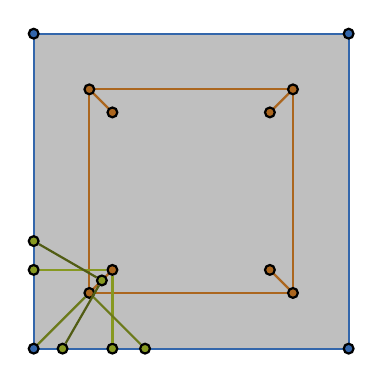
\begin{tikzpicture}[thick]
  \coordinate (p0) at (-2,-2);
  \coordinate (p1) at (2,-2);
  \coordinate (p2) at (2,2);
  \coordinate (p3) at (-2,2);
  \filldraw[fill=lightgray,draw=c0] (p0) -- (p1) -- (p2) -- (p3) -- cycle;%
  \node[point=c0] (m0) at (p0) {};
  \node[point=c0] at (p1) {};
  \node[point=c0] at (p2) {};
  \node[point=c0] at (p3) {};
  \coordinate (q0) at (-1.2929,-1.2929);
  \coordinate (q1) at (1.2929,-1.2929);
  \coordinate (q2) at (1.2929,1.2929);
  \coordinate (q3) at (-1.2929,1.2929);
  \coordinate (q4) at (-1,-1);
  \coordinate (q5) at (1,-1);
  \coordinate (q6) at (1,1);
  \coordinate (q7) at (-1,1);
  \draw[c1] (q0)--(q1);
  \draw[c1] (q1)--(q2);
  \draw[c1] (q2)--(q3);
  \draw[c1] (q3)--(q0);
  \draw[c1] (q0)--(q4);
  \draw[c1] (q1)--(q5);
  \draw[c1] (q2)--(q6);
  \draw[c1] (q3)--(q7);
  \node[point=c1] (n0) at (q0) {};
  \node[point=c1] (n1) at (q1) {};
  \node[point=c1] (n2) at (q2) {};
  \node[point=c1] (n3) at (q3) {};
  \node[point=c1] (n4) at (q4) {};
  \node[point=c1] (n5) at (q5) {};
  \node[point=c1] (n6) at (q6) {};
  \node[point=c1] (n7) at (q7) {};
  %%%
  \node[point=c2] (r0) at (-2,-1) {};
  \node[point=c2] (r1) at (-1,-2) {};
  \node[point=c2] (r2) at (-.5858,-2) {};
  \node[point=c2] (r3) at (-1.134,-1.134) {};
  \node[point=c2] (r4) at (-1.633,-2) {};
  \node[point=c2] (r5) at (-2,-.634) {};
  \draw[c2!100!black] (r0)--(n4)--(r1);
  \draw[c2!80!black] (m0)--(n0)--(r2);
  \draw[c2!60!black] (r4)--(r3)--(r5);
\end{tikzpicture}

  }\,
  \subfloat[$d_1 = 1$, $d_2 = \sqrt{2}$, $\alpha = 90^{\circ}$]{\label{fig:examples:2}
    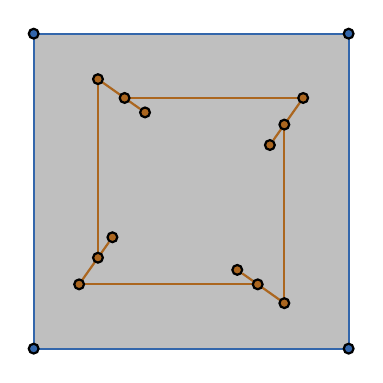
\begin{tikzpicture}[thick]
  % Boundary
  \coordinate (b0) at (-2,-2);
  \coordinate (b1) at (2,-2);
  \coordinate (b2) at (2,2);
  \coordinate (b3) at (-2,2);
  \filldraw[fill=lightgray,draw=c0] (b0) -- (b1) -- (b2) -- (b3) -- cycle;
  \node[point=c0] at (b0) {};
  \node[point=c0] at (b1) {};
  \node[point=c0] at (b2) {};
  \node[point=c0] at (b3) {};
  % Solution segments
  \pgfmathparse{1}\let\da\pgfmathresult
  \pgfmathparse{sqrt(2)}\let\db\pgfmathresult
  \pgfmathparse{pi*0.5}\let\angle\pgfmathresult
  \pgfmathparse{cos(deg(\angle))}\let\c\pgfmathresult
  \pgfmathparse{sqrt(\da*\da+\db*\db-2*\c*\da*\db)}\let\dc\pgfmathresult
  \pgfmathparse{(\dc*\dc-\db*\db+\da*\da)/(2*\dc)}\let\x\pgfmathresult
  \pgfmathparse{sqrt(\da*\da-\x*\x)}\let\y\pgfmathresult
  %
  \coordinate[shift={(-2,-2)}] (a0) at (\x,\y);
  \coordinate[shift={(2-\dc,-2)}] (a1) at (\x,\y);
  \begin{scope}[rotate=90,shift={(-2,-2)}]\coordinate (a2) at (\x,\y);\end{scope}
  \begin{scope}[rotate=90,shift={(2-\dc,-2)}]\coordinate (a3) at (\x,\y);\end{scope}
  \begin{scope}[rotate=180,shift={(-2,-2)}]\coordinate (a4) at (\x,\y);\end{scope}
  \begin{scope}[rotate=180,shift={(2-\dc,-2)}]\coordinate (a5) at (\x,\y);\end{scope}
  \begin{scope}[rotate=270,shift={(-2,-2)}]\coordinate (a6) at (\x,\y);\end{scope}
  \begin{scope}[rotate=270,shift={(2-\dc,-2)}]\coordinate (a7) at (\x,\y);\end{scope}
  \draw[c1] (a0)--(a1);
  \draw[c1] (a2)--(a3);
  \draw[c1] (a4)--(a5);
  \draw[c1] (a6)--(a7);
  \node[point=c1,shift={(-2,-2)}] (a8) at (\da,\db) {};
  \draw[c1] (a0)--(a8);
  \begin{scope}[rotate=90,shift={(-2,-2)}]\node[point=c1] (a9) at (\da,\db) {};\end{scope}
  \draw[c1] (a2)--(a9);
  \begin{scope}[rotate=180,shift={(-2,-2)}]\node[point=c1] (a10) at (\da,\db) {};\end{scope}
  \draw[c1] (a4)--(a10);
  \begin{scope}[rotate=270,shift={(-2,-2)}]\node[point=c1] (a11) at (\da,\db) {};\end{scope}
  \draw[c1] (a6)--(a11);
  % Witnesses
  \begin{scope}[shift={(-2,-2)}]\myWitness\end{scope}
  \begin{scope}[shift={(2-\dc,-2)}]\myWitness\end{scope}
  \begin{scope}[shift={(-2,-2+\dc)},rotate=270]\myWitness\end{scope}
  \begin{scope}[shift={(-2,-2+\db)},rotate=305]\myWitness\end{scope}
  %%
  %% \begin{scope}[shift={(1,-1)},rotate=270]\witness[p1][q1][r1][c2!20!black]\end{scope}
  %% \begin{scope}[shift={(1.06,-.721)},rotate=250]\witness[p2][q2][r2][c2!40!black]\end{scope}
  %% \begin{scope}[shift={(1.2929,-.5858)},rotate=225]\witness[p3][q3][r3][c2!60!black]\end{scope}
  %% \begin{scope}[shift={(1.655,-.717)},rotate=200]\witness[p4][q4][r4][c2!80!black]\end{scope}
  %% \begin{scope}[shift={(2,-1)},rotate=180]\witness[p5][q5][r5][c2!100!black]\end{scope}
  %% %%
  %% \begin{scope}[shift={(-2,2)},rotate=0]\crvb\end{scope}
  %% \begin{scope}[shift={(-2,-2)},rotate=90]\crvb\end{scope}
  %% \begin{scope}[shift={(2,-2)},rotate=180]\crvb\end{scope}
  %% \begin{scope}[shift={(2,2)},rotate=270]\crvb\end{scope}
  %% %%
  \node[point=c1] (n0) at (a0) {};
  \node[point=c1] (n1) at (a1) {};
  \node[point=c1] (n2) at (a2) {};
  \node[point=c1] (n3) at (a3) {};
  \node[point=c1] (n4) at (a4) {};
  \node[point=c1] (n5) at (a5) {};
  \node[point=c1] (n6) at (a6) {};
  \node[point=c1] (n7) at (a7) {};
\end{tikzpicture}

  }\,
  \subfloat[$d_1 = 1$, $d_2 = \sqrt{2}$, $\alpha = 45^{\circ}$]{\label{fig:examples:3}
    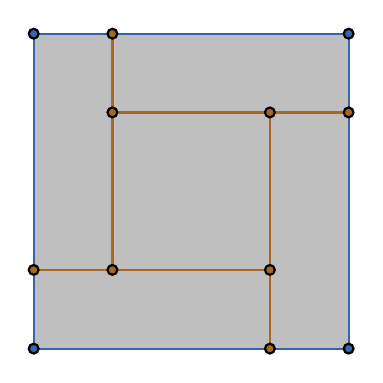
\begin{tikzpicture}[thick]
  \coordinate (p0) at (-2,-2);
  \coordinate (p1) at (2,-2);
  \coordinate (p2) at (2,2);
  \coordinate (p3) at (-2,2);
  \filldraw[fill=lightgray,draw=c0] (p0) -- (p1) -- (p2) -- (p3) -- cycle;%
  \node[point=c0] (m0) at (p0) {};
  \node[point=c0] at (p1) {};
  \node[point=c0] at (p2) {};
  \node[point=c0] at (p3) {};
  \coordinate (a0) at (-2,-1);
  \coordinate (a1) at (1,-1);
  \coordinate (a2) at (1,-2);
  \coordinate (a3) at (1,1);
  \coordinate (a4) at (2,1);
  \coordinate (a5) at (-1,1);
  \coordinate (a6) at (-1,2);
  \coordinate (a7) at (-1,-1);
  \draw[c1] (a0)--(a1);
  \draw[c1] (a2)--(a3);
  \draw[c1] (a4)--(a5);
  \draw[c1] (a6)--(a7);
  %%%
  \begin{scope}[shift={(-1.3,1)}]\sights\end{scope}
  \begin{scope}[shift={(-1,0.5)},rotate=90]\sights\end{scope}
  \begin{scope}[shift={(-1,-1.3)},rotate=90]\sights\end{scope}
  %%
  \begin{scope}[shift={(1,-1)},rotate=270]\sights[p1][q1][r1][c2!20!black]\end{scope}
  \begin{scope}[shift={(1.06,-.721)},rotate=250]\sights[p2][q2][r2][c2!40!black]\end{scope}
  \begin{scope}[shift={(1.2929,-.5858)},rotate=225]\sights[p3][q3][r3][c2!60!black]\end{scope}
  \begin{scope}[shift={(1.655,-.717)},rotate=200]\sights[p4][q4][r4][c2!80!black]\end{scope}
  \begin{scope}[shift={(2,-1)},rotate=180]\sights[p5][q5][r5][c2!100!black]\end{scope}
  %%
  %% \draw plot [smooth] coordinates {(q1)(q2)(q3)(q4)(q5)};
  %% \begin{scope}[shift={(0,0)},rotate=0]\crv\end{scope}
  %% \begin{scope}[shift={(-3,-2)},rotate=90]\crvb\end{scope}
  %% \begin{scope}[shift={(0,0)},rotate=180]\crvb\end{scope}
  %% \begin{scope}[shift={(3,2)},rotate=270]\crvb\end{scope}
  \begin{scope}[shift={(-2,2)},rotate=0]\crvb\end{scope}
  \begin{scope}[shift={(-2,-2)},rotate=90]\crvb\end{scope}
  \begin{scope}[shift={(2,-2)},rotate=180]\crvb\end{scope}
  \begin{scope}[shift={(2,2)},rotate=270]\crvb\end{scope}
  %%
  \node[point=c1] (n0) at (a0) {};
  \node[point=c1] (n1) at (a1) {};
  \node[point=c1] (n2) at (a2) {};
  \node[point=c1] (n3) at (a3) {};
  \node[point=c1] (n4) at (a4) {};
  \node[point=c1] (n5) at (a5) {};
  \node[point=c1] (n6) at (a6) {};
  \node[point=c1] (n7) at (a7) {};
\end{tikzpicture}

  }\,
  \subfloat[$d_1 = 1$, $d_2 = \sqrt{2}$, $\alpha = 180^{\circ}$]{\label{fig:examples:4}
    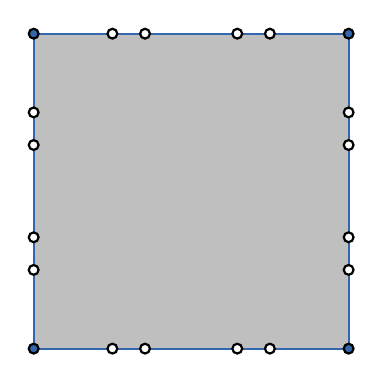
\begin{tikzpicture}[thick]
  % Boundary
  \coordinate (b0) at (-2,-2);
  \coordinate (b1) at (2,-2);
  \coordinate (b2) at (2,2);
  \coordinate (b3) at (-2,2);
  \filldraw[fill=lightgray,draw=c0] (b0) -- (b1) -- (b2) -- (b3) -- cycle;
  \node[point=c0] at (b0) {};
  \node[point=c0] at (b1) {};
  \node[point=c0] at (b2) {};
  \node[point=c0] at (b3) {};
  \begin{scope}[rotate=0,shift={(-2,-2)}]
    \elipricArc{1.4142}{1}
    \elipricArc{1}{1.4142}
    \node[point=white] at (0,1.4142) {};
    \node[point=white] at (1.4142,0) {};
    \node[point=white] at (0,1) {};
    \node[point=white] at (1,0) {};
  \end{scope}
  \begin{scope}[rotate=90,shift={(-2,-2)}]
    \elipricArc{1.4142}{1}
    \elipricArc{1}{1.4142}
    \node[point=white] at (0,1.4142) {};
    \node[point=white] at (1.4142,0) {};
    \node[point=white] at (0,1) {};
    \node[point=white] at (1,0) {};
  \end{scope}
  \begin{scope}[rotate=180,shift={(-2,-2)}]
    \elipricArc{1.4142}{1}
    \elipricArc{1}{1.4142}
    \node[point=white] at (0,1.4142) {};
    \node[point=white] at (1.4142,0) {};
    \node[point=white] at (0,1) {};
    \node[point=white] at (1,0) {};
  \end{scope}
  \begin{scope}[rotate=270,shift={(-2,-2)}]
    \elipricArc{1.4142}{1}
    \elipricArc{1}{1.4142}
    \node[point=white] at (0,1.4142) {};
    \node[point=white] at (1.4142,0) {};
    \node[point=white] at (0,1) {};
    \node[point=white] at (1,0) {};
  \end{scope}
  \pgfmathparse{2.4142}\let\dc\pgfmathresult
  \pgfmathparse{1}\let\x\pgfmathresult
  \pgfmathparse{0}\let\y\pgfmathresult
  \begin{scope}[rotate=-10,shift={(-1.694,-1.905)}]\myWitness\end{scope}
\end{tikzpicture}

  }\,
  \subfloat[$d_1 = 1$, $d_2 = \sqrt{2}$, $\alpha = 45^{\circ}$]{\label{fig:examples:5}
    \begin{tikzpicture}[]
  \coordinate (p0) at (-2,-2);
  \coordinate (p1) at (2,-2);
  \coordinate (p2) at (2,2);
  \coordinate (p3) at (-2,2);
  \filldraw[fill=lightgray,draw=c0] (p0) -- (p1) -- (p2) -- (p3) -- cycle;%
  \node[point=c0] at (p0) {};
  \node[point=c0] at (p1) {};
  \node[point=c0] at (p2) {};
  \node[point=c0] at (p3) {};
  %
  \begin{scope}[shift={(-2,-2)},rotate=0]\obs\end{scope}
  \begin{scope}[shift={(2,-2)},rotate=90]\obs\end{scope}
  \begin{scope}[shift={(2,2)},rotate=180]\obs\end{scope}
  \begin{scope}[shift={(-2,2)},rotate=270]\obs\end{scope}
  %
  \coordinate (r0) at (-0.95,-0.95);
  \coordinate (r1) at (0.95,-0.95);
  \coordinate (r2) at (0.95,0.95);
  \coordinate (r3) at (-0.95,0.95);
  \filldraw[fill=white,draw=c0] (r0) -- (r1) -- (r2) -- (r3) -- cycle;%
  \node[point=c0] at (q0) {};
  \node[point=c0] at (q1) {};
  \node[point=c0] at (q2) {};
  \node[point=c0] at (q3) {};
  %%% Witnesses
  \begin{scope}[shift={(-0.586,-1.293)},rotate=135]\witnessB\end{scope}
  \begin{scope}[shift={(-0.592,-1.234)},rotate=140]\witnessB\end{scope}
  \node[point=c1] at (b) {};
  \begin{scope}[rotate=90]
    \begin{scope}[shift={(-0.592,-1.234)},rotate=140]\node[point=c1] at (1,0) {};\end{scope}
  \end{scope}
  \begin{scope}[rotate=180]
    \begin{scope}[shift={(-0.592,-1.234)},rotate=140]\node[point=c1] at (1,0) {};\end{scope}
  \end{scope}
  \begin{scope}[rotate=270]
    \begin{scope}[shift={(-0.592,-1.234)},rotate=140]\node[point=c1] at (1,0) {};\end{scope}
  \end{scope}
  %
  \begin{scope}[shift={(-0.601,-1.399)},rotate=127]\witnessB\end{scope}
  \node[point=c1] at (b) {};
  \begin{scope}[rotate=90]
    \begin{scope}[shift={(-0.601,-1.399)},rotate=127]\node[point=c1] at (1,0) {};\end{scope}
  \end{scope}
  \begin{scope}[rotate=180]
    \begin{scope}[shift={(-0.601,-1.399)},rotate=127]\node[point=c1] at (1,0) {};\end{scope}
  \end{scope}
  \begin{scope}[rotate=270]
    \begin{scope}[shift={(-0.601,-1.399)},rotate=127]\node[point=c1] at (1,0) {};\end{scope}
  \end{scope}
  %% Solution
  \begin{scope}[shift={(-2,2)},rotate=0]\crvb\end{scope}
  \begin{scope}[shift={(-2,-2)},rotate=90]\crvb\end{scope}
  \begin{scope}[shift={(2,-2)},rotate=180]\crvb\end{scope}
  \begin{scope}[shift={(2,2)},rotate=270]\crvb\end{scope}
  %%
\end{tikzpicture}

  }
  \caption[]{Various examples. The free space is filled with a light-gray color.
    The boundary of the free space is drawn with blue segments.
    Orange curves contains all the possible locations of the sensor.
    Two green segments with a common endpoint shows a witness.}
  \label{fig:examples}
\end{figure}

If only a single measurement is carried out at an unknown direction, the possible locations of the robot comprise two-dimentional regions. Here, we concern ourselves with a variant of the problem where a query consists of three real numbers $d_1$, $\alpha \neq 0$, $d_2$ describing the following sequence of events: The sensor at its original state obtained the distance reading $d_1$, then the sensor was rotated (without translating) by $\alpha$ radians counterclockwise, and then it obtained a second distance reading $d_2$. The possible locations of the robot in this case comprise of one-dimentional curves in the general case; see Figure~\ref{fig:examples}. If the query is augmented by a second rotation followed by a third measurement, the possible locations of the robot consist of one or more isolated points (in the general case).

A more complicated problem allows for a translation of the robot before the second measurement is taken. In this variant a query consists of four real numbers $d_1$, $\alpha$, $t$, $d_2$, where $t$ denotes a translation vector in the plane. If $t \neq 0$, the two measurements can be taken simultaneously. This is possible in practice, if two distinct sensors are at our disposal. We made experiments with a real robot equipped with two sensors.

% =============================================================================
\section{Algebraic Analysis}
\label{sec:analysis}
% =============================================================================

\begin{figure}[!htp]
  \centerline{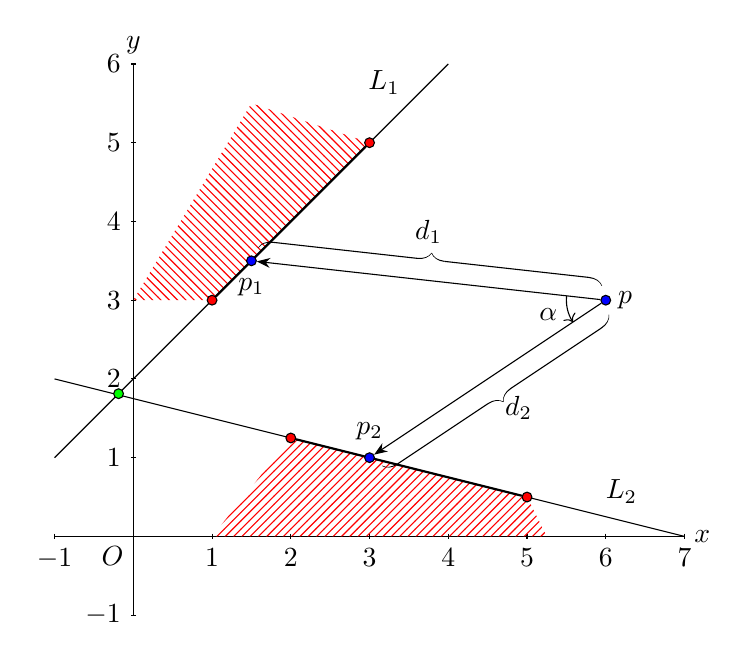
\begin{tikzpicture}[]
    \draw[-] (-1,0) -- (7,0) node[right] {$x$};
    \draw (0,0) node[below left] {$O$};
    \draw[-] (0,-1) -- (0,6) node[above] {$y$};
    \foreach \x in {-1, 1, 2, 3, 4, 5, 6, 7}
      \draw (\x cm,1pt) -- (\x cm,-1pt) node[anchor=north] {$\x$};
      \foreach \y in {-1, 1, 2, 3, 4, 5, 6}
      \draw (1pt,\y cm) -- (-1pt,\y cm) node[anchor=east] {$\y$};
    %
    \coordinate (p21) at (-1,2);
    \coordinate (p22) at (7,0);
    \draw (p21)--(p22) node[pos=0.9,anchor=south,outer sep=3pt]{$L_2$};
    \coordinate (q21) at (5,0.5);
    \coordinate (q22) at (2,1.25);
    \fill[pattern=north east lines,pattern color=red]
      (1,0)--(q22)--(q21)--(5.25,0)--cycle;
    \node[point] (a) at (q21) {};
    \node[point] (b) at (q22) {};
    \draw[thick] (a)--(b);
    %
    \coordinate (p11) at (-1,1);
    \coordinate (p12) at (4,6);
    \draw (p11)--(p12) node[pos=0.9,anchor=south east,outer sep=0pt]{$L_1$};
    \coordinate (q11) at (3,5);
    \coordinate (q12) at (1,3);
    \fill[pattern=north west lines,pattern color=red]
      (1.5,5.5)--(q11)--(q12)--(0,3)--cycle;
    \node[point] (a) at (q11) {};
    \node[point] (b) at (q12) {};
    \draw[thick] (a)--(b);
    %
    \node[point=blue,label={[label distance=-1pt]0:\rotatebox{0}{$p$}}] (p)
      at (6,3) {};
    \node[point=blue,label={[label distance=1pt]90:\rotatebox{0}{$p_2$}}] (p2)
        at (3,1) {};
    \draw[->,>=Stealth] (p)--(p2);
    \draw [decorate,decoration={calligraphic brace,raise=5pt,amplitude=5pt}]
      (p)--(p2) node[midway,anchor=north west,outer sep=3pt]{$d_2$};
    \node[point=blue,label={[label distance=1pt]270:\rotatebox{0}{$p_1$}}] (p1)
      at (1.5,3.5) {};
    \draw[->,>=Stealth] (p)--(p1);
    \draw [decorate,decoration={calligraphic brace,raise=5pt,amplitude=5pt}]
      (p1)--(p) node[midway,anchor=south,outer sep=10pt]{$d_1$};
    \pic [draw,->,"$\alpha$",angle eccentricity=1.5] {angle=p1--p--p2};
    \node [point=green] at (-0.1875,1.8125) {};
  \end{tikzpicture}}
  \caption{Local view of the problem.}
  \label{fig:analysis}
\end{figure}

We start with an algebraic analysis of the problem. Here, we concentrate at a local view of the problem, where we only consider two walls (edges) of obstacles and ignore everything else; see Figure~\ref{fig:analysis}. Let $L_1: a_1 x + b_1 y + c_1 = 0$ and $L_2: a_2 x + b_2 y + c_2 = 0$ denote the two underlying lines of the two edges of obstacles hit by the two measuring rays, respectively. Let $p = (x,y)$ denote a point in the workspace our sensor could be located at. Let $p_1 = (x_1,y_1)$ denote the point on $L_1$ hit by the first measuring ray, and similarly, let $p_2 = (x_2,y_2)$ denote the point on $L_2$ hit by the second measuring ray. Employing the law of cosine (Equation~\ref{eq:loc}), the following equations must be satisfied:
\begin{gather}
  a_1\cdot x_1 + b_1\cdot y_1 + c1 = 0\\
  a_2\cdot x_2 + b_2\cdot y_2 + c_2 = 0\\
  |p - p_1| = d_1\\
  |p - p_2| = d_2\\
  d_1^2 + d_2^2 + 2\cdot \cos(\alpha)\cdot d_1\cdot d_2 = |p_1 - p_2|^2\label{eq:loc}
\end{gather}
In the degenerate case, where $L_1$ and $L_2$ are parallel (or $L_1 == L_2$) the loci of all points that satisfy the above equations form a line. This line must be trimmed to a segment according to the actual edge lengths and interiors of the obstacles. In all other cases the loci of points form two ellipses that correspond to clockwise and counter clockwise rotations. The ellipse that corresponds to the clockwise location is discarded and the other must be trimmed to obtain that actual possible locations.

Solving the above non-linear equation system is messy. We can add some constraints to the above system without compromising. First, we translate the scene, by setting $c_1 = 0$, $c_2 = 0$, coercing the intersection point of $L_1$ and $L_2$ to be at the origin. Then, we rotate the scene, setting $a_1 = 0$, coercing $L_1$ to lie on the $x$-axis. Once we find the desired elliptic arc in our transformed space, we can apply an inverse rotation followed by an inverse translation to obtain the elliptic arc in the original space.

First, we handle the simple case, where $b_2 = 0$. Recall that $L_1$ lies on the $x$-axis. This additional constraint implies that $L_2$ lies on the $y$-axis. ($L_1$ and $L_2$ are orthogonal.) Manipulating the system equation above and employing Matlab to simplify the equations above, we obtain the single equation:
\begin{equation}
  d_1^4\cdot x^4 + (4\cdot k^2 - 2\cdot d_1^2\cdot d_2^2)\cdot x^2\cdot y^2 - 2\cdot d_1^2\cdot k^2\cdot x^2 + d_2^4\cdot y^4 - 2\cdot d_2^2\cdot k^2\cdot y^2 + k^4 = 0\label{eq:polynomial-orthogonal-x-aligned},
\end{equation}
where $k = \cos(\alpha)\cdot d_1\cdot d_2$. Let $P_1$ denote the bivariate polynomial on the left hand side of Equation~\ref{eq:polynomial-orthogonal-x-aligned}. The zero set of $P_1$ represents the two desired ellipses. Employing Matlab yet again to factorize the polynomial $P_1$, we get: $P_1: (A_1\cdot x^2 + B_1\cdot y^2 + C_1\cdot x\cdot y + D_1)\cdot (A_2\cdot x^2 + B_2\cdot y^2 + C_2\cdot x\cdot y +D_2)$, where
\begin{minipage}[c]{0.5\linewidth}
\begin{align*}
  A_1 &= d_1^2\\
  B_1 &= d_2^2\\
  C_1 &= 2(d_1^2\cdot d_2^2 - k^2)(1/2)\\
  D_1 &= -k^2
\end{align*}
\end{minipage}
\begin{minipage}[c]{0.5\linewidth}
\begin{align*}
  A_2 &= d_1^2\\
  B_2 &= d_2^2\\
  C_2 &= -2(d_1^2\cdot d_2^2 - k^2)(1/2)\\
  D2 &= -k^2
\end{align*}
\end{minipage}
You can visualize the ellipses and how they dynamically change as a
consequence of changing the parameters $d_1$, $\alpha$, $d_2$ using
the GeoGebra\footnote{\url{https://www.geogebra.org}} online tool;
download the GeoGebra script
\url{https://www.geogebra.org/calculator/rvqwxqcd} and upload in
GeoGebra. Second, we denote $m_2 = \frac{a_2}{b_2}$, assuming the
lines are not parallel. The obtained polynomial, $P_2$, in this case
is much more complex; see~\ref{ssec:derivation-p2}. Use the GeoGebra
script \url{https://www.geogebra.org/calculator/ferztmgh} to visualize
the ellipses in this case.

% =============================================================================
\section{Derivation}
\label{sec:derivation}
% =============================================================================
We repeat the system equation in the general case:
\begin{align}
  a_1 x_1 + b_1 y_1 + c_1 &= 0\\
  a_1 x_2 + b_1 y_2 + c_1 &= 0\\
  (x - x_1)^2 + (y - y_1)^2 &= d_1^2\label{eq:1}\\
  (x - x_2)^2 + (y - y_2)^2 &= d_2^2\label{eq:2}\\
  (x_2 - x_1)^2 + (y_2 - y_1)^2 &= d_1^2 + d_2^2 - 2 c d_1 d_2 = d_1^2 + d_2^2 - 2 k\label{eq:3}
\end{align}

% -----------------------------------------------------------------------------
\subsection{Constraining the Slopes of Both Lines}
\label{ssec:derivation-constraining-slopes}
% -----------------------------------------------------------------------------
We set $y_1 = 0$ and $x_2 = 0$, coercing $L_1$ and $L_2$ to lie on the
$x$- and $y$-axes, respectively.
Equations~\ref{eq:1},~\ref{eq:2}, and~\ref{eq:3} reduce to:
\begin{align}
  (x - x_1)^2 + y^2 &= d_1^2\label{eq:d1-oa}\\
  x^2 + (y - y_2)^2 &= d_2^2\label{eq:d2-oa}\\
  x_1^2 + y_2^2 &= d_1^2 + d_2^2 - 2 k\label{eq:d-oa}
\end{align}

\noindent
We substitute $d_1$ and $d_2$ in Equation~\ref{eq:d-oa} and obtain the single equation:
\begin{align}
  x^2 + y^2 - x x_1 - y y_2 - k &= 0\label{eq:s-oa}
\end{align}

\noindent
We introduce the symbols $s_1$ and $s_2$, and get
\begin{align*}
  x_1 &= x \pm \sqrt{s_1}\\
  y_2 &= y \pm \sqrt{s_2},
\end{align*}
where
\begin{align*}
  s_1 &= d_1^2 - y^2\\
  s_2 &= d_2^2 - x^2
\end{align*}

\noindent
We substitute $x_1$ and $x_2$ in Equation~\ref{eq:s-oa} and get:
\begin{align*}
  x^2 + y^2 - x (x \pm \sqrt{s_1}) - y (y \pm \sqrt{s_2}) - k &= 0
\end{align*}

\noindent
We expand and exchange and get:
\begin{align*}
  \pm x \sqrt{s_1} \pm y \sqrt{s_2} &= k
\end{align*}

\noindent
We raise to the power of two each side and get:
\begin{align*}
  x^2 s_1 + y^2 s_2 + 2 x y \sqrt{s_1 s_2} &= k^2
\end{align*}

\noindent
We exchange and get:
\begin{align*}
  2 x y \sqrt{s_1 s_2} &= k^2 - x^2 s_1 - y^2 s_2
\end{align*}

\noindent
We raise again and get:
\begin{align*}
  4 x^2 y^2 s_1 s_2 &= (k^2 - x^2 s_1 - y^2 s_2)^2
\end{align*}

\noindent
We expand and get:
\begin{align*}
  4 x^2 y^2 s_1 s_2 &= k^4 + x^4 s_1^2 + y^4 s_2^2 - 2 k^2 x^2 s_1 - k^2 y^2 s_2 + 2 x^2 y^2 s_1 s_2
\end{align*}

\noindent
We exchange and substitute $s_1$ and $s_2$ and get:
\begin{align*}
  k^4 + x^4 (d_1^2 - y^2)^2 + y^4 (d_2^2 - x^2)^2 - 2 k^2 x^2 (d_1^2 - y^2) - k^2 y^2 (d_2^2 - x^2) - 2 x^2 y^2 (d_1^2 - y^2) (d_2^2 - x^2) &= 0\\
\end{align*}

\noindent
We expand and regroup and get:
\begin{align}
  d_1^4 x^4 + y^2 x^2 (4 k^2 - 2 d_1^2 d_2^2) - 2 d_1^2 k^2 x^2 + d_2^4 y^4 - 2 d_2^2 k^2 y^2 + k^4 &= 0
\end{align}

% -----------------------------------------------------------------------------
\subsection{Constraining the Intersection Point}
\label{ssec:derivation-constraining-origin}
% -----------------------------------------------------------------------------
\setlength{\parskip}{1ex}
%\noindent
We set $c_1 = c_2 = 0$, coercing the intersection point of $L_1$ and $L_2$ to coincide with the origin, and denote $m_1 = \frac{a_1}{b_1}$ and $m_2 = \frac{a_2}{b_2}$; we get $y_1 = m_1 x_1$ and $y_2 = m_2 x_2$.

\noindent
We substitute $y_1$ and $y_2$ in equations~\ref{eq:1}, \ref{eq:2}, and \ref{eq:3} and get:
\begin{align}
  (x - x_1)^2 + (y - m_1 x_1)^2 & = d_1^2\\
  (x - x_2)^2 + (y - m_2 x_2)^2 & = d_2^2\\
  (x_2 - x_1)^2 + (m_2 x_2 - m_1 x_1)^2 & = d_1^2 + d_2^2 - 2 k
\end{align}

\noindent
We expand and regroup and get:
\begin{align}
  %x^2 + x_1^2 - 2 x x_1 + y^2 + m_1^2x_1^2 - 2 m_1 y x_1 &= d_1^2\\
  (1 + m_1^2) x_1^2 - 2 (x + m_1 y) x_1  + x^2 + y^2  &= d_1^2\label{eq:d1}\\
  (1 + m_2^2) x_2^2 - 2 (x + m_2 y) x_2  + x^2 + y^2  &= d_2^2\label{eq:d2}\\
  % x_2^2 + x_1^2 - 2 x_1 x_2 + m_1^2 x_1^2 + m_2^2 x_2^2 - 2 m_1 m_2 x_1 x_2 &= d_1^2 + d_2^2 - 2 k\\
  (1 + m_1^2) x_1^2 + (1 + m_2^2) x_2^2 - 2 (1 + m_1 m_2) x_1 x_2 &= d_1^2 + d_2^2 - 2 k\label{eq:d}
\end{align}

\noindent
We substitute $d_1$ and $d_2$ in Equation~\ref{eq:d} and obtain the single equation:
\begin{align}
  % 2 (1 + m_1 m_2) x_1 x_2 - 2 (x + m_1 y) x_1 - 2 (x + m_2 y) x_2 + 2 x^2 + 2 y^2 &= 2 k\\
  (1 + m_1 m_2) x_1 x_2 - (x + m_1 y) x_1 - (x + m_2 y) x_2 + x^2 + y^2 - k &= 0\label{eqs}
\end{align}

\noindent
We introduce the symbols $r_1$, $s_1$, $r_2$, and $s_2$, and get
\begin{align*}
  x_1 &= r_1 \pm \sqrt{s_1}\\
  x_2 &= r_2 \pm \sqrt{s_2},
\end{align*}
where
\begin{align*}
  r_1 &= ((x + m_1 y) / (1 + m_1^2))\\
  s_1 &= (((x + m_1 y)^2 - (1 + m_1^2) (x^2 + y^2 - d_1^2)) / (1 + m_1^2)^2)\\
  r_2 &= ((x + m_2 y) / (1 + m_2^2))\\
  s_2 &= (((x + m_2 y)^2 - (1 + m_2^2) (x^2 + y^2 - d_2^2)) / (1 + m_2^2)^2)
\end{align*}

\noindent
We substitute $x_1$ and $x_2$ in Equation~\ref{eqs} and get:
\begin{align*}
(1 + m_1 m_2) (r_1 + \sqrt{s_1}) (r_2 + \sqrt{s_2}) - (x + m_1 y) (r_1 + \sqrt{s_1}) - (x + m_2 y) (r_2 + \sqrt{s_2}) + x^2 + y^2 - k &= 0
\end{align*}

\noindent
We expand and regroup and get:
\begin{multline*}
  (1 + m_1 m_2) r_1 r_2
  + (1 + m_1 m_2) r_1 \sqrt{s_2}
  + (1 + m_1 m_2) r_2 \sqrt{s_1}
  + (1 + m_1 m_2) \sqrt{s_1 s_2})\\
  - \sqrt{s_1} (x + m_1 y)
  - \sqrt{s2} (x + m_2 y)
  - r_1 (x + m_1 y) - r_2 (x + m_2 y) + x^2 + y^2 - k = 0
\end{multline*}

\noindent
We exchange and get:
\begin{align*}
  \sqrt{s_1} (r_2 \ell - x - m_1 y) + \sqrt{s_2} (r_1 \ell - x - m_2 y) &=
  r1 (x + m_1 y) + r_2 (x + m_2 y) - x^2 - y^2 + k - \ell r_1 r_2 - \sqrt{s_1 s_2} \ell,
\end{align*}
where $\ell = 1 + m_1 m_2$.

\noindent
We raise to the power of two each side and get:
\begin{multline*}
  s_1 (r_2 \ell - x - m_1 y)^2 + s_2 (r_1 \ell - x - m_2 y)^2 +
      2 \sqrt{s_1 s_2} (r_2 \ell - x - m_1 y) (r_1 \ell - x - m_2 y) = \\
  (r_1 (x + m_1 y) + r_2 (x + m_2 y) - x^2 - y^2 + k - \ell (r_1 r_2))^2 + \ell^2 s_1 s_2 -\\
      2 \sqrt{s_1 s_2} \ell (r_1 (x + m_1 y) + r_2 (x + m_2 y) - x^2 - y^2 + k - \ell (r_1 r_2))
\end{multline*}

\noindent
We exchange and get:
\begin{multline*}
  2 \sqrt{s_1 s_2} ((r_2 \ell - x - m_1 y) (r_1 \ell - x - m_2 y) +
    \ell (r_1 (x + m_1 y) + r_2 (x + m_2 y) - x^2 - y^2 + k - \ell r_1 r_2)) =\\
  (r_1 (x + m_1 y) + r_2 (x + m_2 y) - x^2 - y^2 + k - \ell r_1 r_2)^2 + \ell^2 s_1 s_2 -
      s_1 (r_2 \ell - x - m_1 y)^2 - s_2 (r_1 \ell - x - m_2 y)^2
\end{multline*}

\noindent
We raise again and get:
\begin{multline}
  4 s_1 s_2 ((r_2 \ell - x - m_1 y) (r_1 \ell - x - m_2 y) + \ell (r_1 (x + m_1 y) + r_2 (x + m_2 y) - x^2 - y^2 + k - \ell r_1 r_2))^2 =\\
  ((r_1 (x + m_1 y) + r_2 (x + m_2 y) - x^2 - y^2 + k - \ell r_1 r_2)^2 + \ell^2 s_1 s_2 -
    s_1 (r_2 \ell - x - m_1 y)^2 - s_2 (r_1 \ell - x - m_2 y)^2)^2\label{eq:g}
\end{multline}

% -----------------------------------------------------------------------------
\subsection{Constraining the Slope of One Line}
\label{ssec:derivation-constraining-slope}
% -----------------------------------------------------------------------------
We set $m_1 = 0$, which implies that $\ell = 1$, in
Equation~\ref{eq:g}, coercing $L_1$ to lie on the $x$-axis, and get:
\begin{multline*}
  4 s_1 s_2 ((r_2 - x - m_1 y) (r_1 - x - m_2 y) + (r_1 (x + m_1 y) + r_2 (x + m_2 y) - x^2 - y^2 + k - r_1 r_2))^2 =\\
  ((r_1 (x + m_1 y) + r_2 (x + m_2 y) - x^2 - y^2 + k - r_1 r_2)^2 + s_1 s_2 -
    s_1 (r_2 - x - m_1 y)^2 - s_2 (r_1 - x - m_2 y)^2)^2
\end{multline*}
We simplify the resutimg equation using Matlab. We obtain the
bivariate polynomial $P_2$, the zero set of which represents the
points satisfying the equation. We employ Matlab yet again to
factorize the polynomial $P_2$; see Section~\ref{ssec:derivation-pa}
for the final expressions. The Matlab script is available at
\url{http://acg.cs.tau.ac.il/projects/in-house-projects/localization-with-few-distance-measurements/solution.m}.

%% % -----------------------------------------------------------------------------
%% \subsection{Constraining the Two Lines to be Orthogonal}
%% \label{ssec:derivation-constraining-orthogonal}
%% % -----------------------------------------------------------------------------
%% If the $L_1$ and $L_2$ are orthogonal $m_1 m_2 = -1$. It implies that $\ell = 0$.
%% We set $\ell = 0$ in Equation~\ref{eq:g}, coercing $L_1$ and $L_2$ to be
%% orthogonal, and get:
%% \begin{multline*}
%%   4 s_1 s_2 ((x + m_1 y) (x + m_2 y))^2 =
%%   ((r_1 (x + m_1 y) + r_2 (x + m_2 y) - x^2 - y^2 + k)^2 - s_1 (x + m_1 y)^2 - s_2 (x + m_2 y)^2)^2
%% \end{multline*}

%% We simplify the resutimg equation using Matlab. We obtain the
%% bivariate polynomial $P$, the zero set of which represents the
%% points satisfying the equation. We employ Matlab yet again to
%% factorize the polynomial $P$; see Section~\ref{ssec:derivation-po}
%% for the final expressions.

% -----------------------------------------------------------------------------
\subsection{The Result}
\label{ssec:derivation-p2}
% -----------------------------------------------------------------------------
The bivariate polynomial obtained by simplifying the system equation in the case where $L_1$ lies on the $x$-axis and and the intersection point of $L_1$ and $L_2$ coincides with the origin follows.

\begin{alignat*}{3}
  & P_2 && : && 4 \cdot k^2 \cdot y^4
    - 4 \cdot k^3 \cdot y^2
    + k^4 + d_1^4 \cdot d_2^4
    + 2 \cdot k^4 \cdot m_2^2
    + k^4 \cdot m_2^4
    + d_1^4 \cdot y^4
    + d_2^4 \cdot y^4 -\\
  & && && 4 \cdot d_1^2 \cdot k \cdot y^4
    - 4 \cdot d_2^2 \cdot k \cdot y^4
    - 2 \cdot d_1^2 \cdot d_2^2 \cdot k^2
    + 2 \cdot d_1^2 \cdot d_2^2 \cdot y^4
    - 2 \cdot d_1^2 \cdot d_2^4 \cdot y^2 -\\
  & && && 2 \cdot d_1^4 \cdot d_2^2 \cdot y^2
    + 2 \cdot d_1^2 \cdot k^2 \cdot y^2
    + 2 \cdot d_2^2 \cdot k^2 \cdot y^2
    + d_1^4 \cdot m_2^4 \cdot x^4
    + 2 \cdot d_2^4 \cdot m_2^2 \cdot y^4 +\\
  & && && d_2^4 \cdot m_2^4 \cdot y^4
    - 4 \cdot k^3 \cdot m_2^2 \cdot y^2
    + 4 \cdot k^2 \cdot m_2^2 \cdot y^4
    + 4 \cdot d_1^2 \cdot d_2^2 \cdot k \cdot y^2 - \\
  & && && 4 \cdot d_2^2 \cdot k \cdot m_2^2 \cdot y^4
    - 4 \cdot d_1^4 \cdot m_2^3 \cdot x^3 \cdot y
    - 8 \cdot k^2 \cdot m_2^3 \cdot x \cdot y^3
    - 2 \cdot d_1^2 \cdot d_2^2 \cdot k^2 \cdot m_2^2 +\\
  & && && 4 \cdot k^3 \cdot m_2 \cdot x \cdot y
    - 2 \cdot d_1^4 \cdot d_2^2 \cdot m_2^2 \cdot x^2
    - 2 \cdot d_1^2 \cdot d_2^2 \cdot m_2^2 \cdot y^4
    - 2 \cdot d_1^2 \cdot d_2^4 \cdot m_2^2 \cdot y^2+\\
  & && && 2 \cdot d_1^2 \cdot k^2 \cdot m_2^2 \cdot x^2
    - 2 \cdot d_1^2 \cdot k^2 \cdot m_2^4 \cdot x^2
    - 2 \cdot d_1^2 \cdot k^2 \cdot m_2^2 \cdot y^2
    - 2 \cdot d_2^2 \cdot k^2 \cdot m_2^4 \cdot y^2 +\\
  & && && 6 \cdot d_1^4 \cdot m_2^2 \cdot x^2 \cdot y^2
    + 4 \cdot k^2 \cdot m_2^2 \cdot x^2 \cdot y^2
    + 4 \cdot k^2 \cdot m_2^4 \cdot x^2 \cdot y^2
    - 4 \cdot d_1^4 \cdot m_2 \cdot x \cdot y^3 -\\
  & && && 8 \cdot k^2 \cdot m_2 \cdot x \cdot y^3
    + 4 \cdot k^3 \cdot m_2^3 \cdot x \cdot y
    + 4 \cdot d_1^2 \cdot d_2^2 \cdot m_2^3 \cdot x \cdot y^3
    - 12 \cdot d_1^2 \cdot k \cdot m_2^2 \cdot x^2 \cdot y^2 +\\
  & && && 4 \cdot d_1^4 \cdot d_2^2 \cdot m_2 \cdot x \cdot y
    - 4 \cdot d_1^2 \cdot k^2 \cdot m_2 \cdot x \cdot y
    + 12 \cdot d_1^2 \cdot k \cdot m_2 \cdot x \cdot y^3 +\\
  & && && 4 \cdot d_2^2 \cdot k \cdot m_2 \cdot x \cdot y^3
    + 2 \cdot d_1^2 \cdot d_2^2 \cdot m_2^2 \cdot x^2 \cdot y^2
    - 2 \cdot d_1^2 \cdot d_2^2 \cdot m_2^4 \cdot x^2 \cdot y^2 -\\
  & && && 4 \cdot d_1^2 \cdot d_2^2 \cdot m_2 \cdot x \cdot y^3
    + 4 \cdot d_1^2 \cdot k^2 \cdot m_2^3 \cdot x \cdot y
    + 4 \cdot d_1^2 \cdot k \cdot m_2^3 \cdot x^3 \cdot y +\\
  & && && 4 \cdot d_2^2 \cdot k \cdot m_2^3 \cdot x \cdot y^3
    + 8 \cdot d_1^2 \cdot d_2^2 \cdot k \cdot m_2^2 \cdot y^2
    - 8 \cdot d_1^2 \cdot d_2^2 \cdot k \cdot m_2^3 \cdot x \cdot y -\\
  & && && 4 \cdot d_1^2 \cdot d_2^2 \cdot k \cdot m_2 \cdot x \cdot y\\
  & && =\quad && (A_1\cdot x^2 + B_1\cdot y^2 + C_1\cdot x \cdot y + D_1)\cdot
    (A_2\cdot x^2 + B_2\cdot y^2 + C_2\cdot x \cdot y + D_2),\\
  \end{alignat*}
%
where\\
\begin{minipage}[c]{0.5\textwidth}
\begin{align*}
  A_1 &= d_1^2\cdot m_2^2\\
  B_1 &= d_1^2+d_2^2-2\cdot k+d_2^2\cdot m_2^2+2\cdot m_2\cdot e\\
  C_1 &= 2\cdot m_2\cdot (k - d_1^2 - m_2\cdot e)\\
  D_1 &= k^2 - d_1^2\cdot d_2^2 - k^2\cdot m_2^2 - 2\cdot k\cdot m_2\cdot e\\
\end{align*}
\end{minipage}
%
\begin{minipage}[c]{0.5\textwidth}
\begin{align*}
  A_2 &= d_1^2\cdot m_2^2\\
  B_2 &= d_1^2 - 2\cdot k + d_2^2 + d_2^2\cdot m_2^2 - 2\cdot m_2\cdot  e\\
  C_2 &= 2\cdot m_2\cdot (k - d_1^2 + m_2\cdot  e)\\
  D_2 &= k^2 - d_1^2\cdot d_2^2 - k^2\cdot m_2^2 + 2\cdot k\cdot m_2\cdot e\\
\end{align*}
\end{minipage}
and $e = \sqrt{d_1^2\cdot d_2^2 - k^2}$.

\end{document}
